\newif\ifsolutions
\solutionstrue % Show solutions
%\solutionsfalse % Hide solutions

\documentclass{article}
\usepackage{geometry}
\geometry{margin=1in}
\usepackage{tikz}
\usepackage{amssymb}

% fleqn allows setting indent of display math
\usepackage[fleqn]{amsmath}
\setlength{\mathindent}{0pt} % Set indent
% Disable equation numbering (https://tex.stackexchange.com/a/360378)
\makeatletter
\renewcommand\tagform@[1]{}
\makeatother

% Allow Unicode (some, e.g., © and £ at least)
% https://tex.stackexchange.com/questions/370278/is-there-any-reason-to-use-inputenc
\usepackage[utf8]{inputenc}

% Hyperlinks
\usepackage{hyperref}
\hypersetup{colorlinks=true, urlcolor=blue, linkcolor=blue}

% Prevent indentation of paragraphs
\setlength\parindent{0pt}
\setlength{\parskip}{\baselineskip}

% Spacing above/below equations
% https://tex.stackexchange.com/a/69678
\AtBeginDocument{%
 \abovedisplayskip=-\parskip
 \abovedisplayshortskip=-\parskip
 \belowdisplayskip=0pt
 \belowdisplayshortskip=0pt
}

% Allow 3 additional subsection levels
% https://tex.stackexchange.com/a/60212
\usepackage{titlesec}
\setcounter{secnumdepth}{6}
% H4 in HTML
\titleformat{\paragraph}{\normalfont\normalsize\bfseries}{\theparagraph}{1em}{}
\titlespacing*{\paragraph}{0pt}{3.25ex plus 1ex minus .2ex}{1.5ex plus .2ex}
% H5 in HTML
\titleformat{\subparagraph}{\normalfont\normalsize\bfseries}{\thesubparagraph}{1em}{}
\titlespacing*{\subparagraph}{0pt}{3.25ex plus 1ex minus .2ex}{1.5ex plus .2ex}
% H6 in HTML
\titleformat{\subsubparagraph}{\normalfont\normalsize\bfseries}{\thesubsubparagraph}{1em}{}
\titlespacing*{\subsubparagraph}{0pt}{3.25ex plus 1ex minus .2ex}{1.5ex plus .2ex}

% So enumerate at all levels is numbers
% https://tex.stackexchange.com/questions/78842/nested-enumeration-numbering
\renewcommand{\labelenumii}{\arabic{enumii}.}
\renewcommand{\labelenumiii}{\arabic{enumiii}.}
\renewcommand{\labelenumiv}{\arabic{enumiv}.}

\renewcommand{\mbox}{\text}
\newcommand{\ds}[0]{\displaystyle}
\newcommand{\ihat}[0]{\hat{\boldsymbol{\imath}}}
\newcommand{\jhat}[0]{\hat{\boldsymbol{\jmath}}}
\newcommand{\khat}[0]{\hat{\boldsymbol{k}}}
\newcommand{\xhat}[0]{\hat{\mathbf{x}}}
\newcommand{\yhat}[0]{\hat{\mathbf{y}}}
\newcommand{\zhat}[0]{\hat{\mathbf{z}}}
\newcommand{\rhat}[0]{\hat{\mathbf{r}}}
\newcommand{\bfvec}[1]{\vec{\mathbf{#1}}}
\newcommand{\bfcdot}[0]{\boldsymbol{\cdot}}

\usepackage{fancyhdr}
\pagestyle{fancy}
\lhead{Electric Field and r^}
\rhead{\thepage}
\fancyfoot{}

\begin{document}

\section{Overview}

This activity covers topics in Section 21.4 of Young and Freedman 2015, 14th Edition.

The electric field vector, $\bfvec{E}$, is a quantity assigned to a point in space. Given this quantity, we can compute the force on a charge $Q$ will experience if it is placed at that point using the equation $\bfvec{F}=Q\bfvec{E}$. The direction of $\bfvec{E}$ is also the direction a charge will begin to move if released from rest.

To find $\bfvec{E}$ at any point in space, 
compute the force $\bfvec{F}$ due to all other charges on a hypothetical (or ``test") charge $q_o$ at a point where you want to know $\bfvec{E}$. To find $\bfvec{E}$ at that point, divide $\bfvec{F}$ by $q_o$.

\begin{equation}
\bfvec{E} = \frac{\bfvec{F}}{q_o}
\end{equation}

%To find $\bfvec{F}$ when a different charge $Q$ is placed where $q$ was, multiply $\bfvec{E}$ by $Q$.

\section{Example I}

Charge $q_1$ is at $(x,y)=(-a,-a)$. Find the electric field at $(x,y)=(a,a)$ in the form $\bfvec{E}=E_x\ihat + E_y\jhat$. Also, find $E$. (Note that $E$ and $|\bfvec{E}|$ are used interchangebly.)

\textbf{Solution}

To find the electric field at a point in space, we put a hypothetical ``test" charge $q_o$ at that point, compute the force on it due to all other charges, and then use

\begin{equation}
\bfvec{E} = \frac{\bfvec{F}}{q_o}
\end{equation}

The force a positive charge $q_1$ at $(x,y)=(-a,-a)$ exerts on a positive charge $q_2$ at $(x,y)=(a, a)$ was computed in a previous activity.

\begin{equation}
\bfvec{F}_{q_1\text{ on } q_2}=k\frac{|q_1q_2|}{8a^2}(\cos 45^\circ \ihat + \sin 45^\circ \jhat)
\end{equation}

We also found that this equation applies when $q_1$ and $q_2$ are both positive or both are negative. If $q_1$ was positive and $q_2$ was negative, or vice-versa, we found the sign changed:

\begin{equation}
\bfvec{F}_{q_1\text{ on } q_2}=-k\frac{|q_1q_2|}{8a^2}(\cos 45^\circ \ihat + \sin 45^\circ \jhat)
\end{equation}

Based on this, we can write a single equation for all possibilities:

\begin{equation}
\bfvec{F}_{q_1\text{ on } q_2}=k\frac{q_1q_2}{8a^2}(\cos 45^\circ \ihat + \sin 45^\circ \jhat)
\end{equation}

If we replace $q_2$ with $q_o$, this is

\begin{equation}
\bfvec{F}_{q_1\text{ on } q_o}=k\frac{q_1q_o}{8a^2}(\cos 45^\circ \ihat + \sin 45^\circ \jhat)
\end{equation}

The electric field at the location of $q_o$ is then 

$\ds\bfvec{E}_{\text{at }(a,a) \text{ due to }q_1} = \frac{\bfvec{F}}{q_o} = \frac{kq_1}{8a^2}(\cos 45^\circ \ihat + \sin 45^\circ \jhat) =\frac{kq_1}{8a^2}\left[\frac{1}{\sqrt{2}}\ihat + \frac{1}{\sqrt{2}}\jhat\right]$,

where the fact that $\sin 45^\circ=\cos 45^\circ=1/\sqrt{2}$ was used. The magnitude is $E=\sqrt{E_x^2+E_y^2}=k|q_1|/8a^2$.

Sign check: When computing electric fields and forces, it is easy to make a sign error. The electric field vector points in the direction a positive charge will move if released there from rest. Suppose $q_1$ is positive. Our equation predicts that a positive charge released from rest at $(a, a)$ will move up and to the right. Suppose $q_1$ is negative. Our equation predicts that a positive charge will move down and to the left. This is consistent with the fact that like charges repel and unlike charges attract.

\section{Problem I}

Charge $q_1$ is at $(x,y)=(-a,a)$. At $(x,y)=(a, 0)$, find $\bfvec{E}$ in the form $\bfvec{E}=E_x\ihat + E_y\jhat$. Check signs of the components of $\bfvec{E}$ using the technique used in Example I. Also, find $E$.

\input{../Electric_Force/figures/grid.tikz}

\ifsolutions
{\bf Answer}:

From Problem II on the Electric Force Activity, if $q_2$ is at $(x,y)=(a, 0)$ (and using the arguments in the previous example to drop the absolute value sign),

\begin{equation}
\bfvec{F}_{q_1\text{ on } q_2}=k\frac{q_1q_2}{5a^2}\left(\frac{2}{\sqrt{5}}\ihat -\frac{2}{\sqrt{5}}\jhat\right)
\end{equation}

Replacing $q_2$ with a test charge $q_o$,

\begin{equation}
\bfvec{F}_{q_1\text{ on } q_o}=k\frac{q_1q_o}{5a^2}\left(\frac{2}{\sqrt{5}}\ihat -\frac{2}{\sqrt{5}}\jhat\right)
\end{equation}

$\ds\bfvec{E}_{\text{at }(a,0) \text{ due to }q_1} = \frac{\bfvec{F}}{q_o}=\frac{kq_1}{5a^2}\left(\frac{2}{\sqrt{5}}\ihat -\frac{2}{\sqrt{5}}\jhat\right)$
\fi

\newpage

\section{The $\rhat$ Unit Vector}

Previously, when computing the electric force between two charges, you used the formula $F=k{|q_1q_2|}/{r^2}$ to find the magnitude of the force and then used a diagram to write $\bfvec{F}$ in the form $\bfvec{F}=F_x\ihat + F_y\jhat$. A similar process was used for computing $\bfvec{E}$ above (because we calculated $\bfvec{F}$ as part of the process). The textbook provides an equation for the electric field that requires a slightly different calculation method.

The equation for the electric field using a unit vector is

\begin{equation}
\bfvec{E}_{\text{due to }q_1}=kq_1\frac{\rhat}{r^2}\thinspace,
\end{equation}

where $\rhat$ is the unit vector that points from the position of $q_1$ to the point in space where we want to know $\bfvec{E}$, and $r$ is the distance between $q_1$ and that point.

To find $\rhat$, 

\begin{enumerate}

  \item draw a vector, $\bfvec{r}$ from $q_1$ to the point in space where you want to know $\bfvec{E}$;

  \item Write $\bfvec{r}$ in the form $\bfvec{r}=r_x\ihat+r_y\jhat$; then

  \item $\rhat=\bfvec{r}/r$, where $r=\sqrt{r_x^2+r_y^2}$.

\end{enumerate}

\section{Example II}

If $q_1$ is at $(x,y)=(-a,-a)$, find the electric field at $(x,y)=(a,a)$ using $\bfvec{E}_{\text{due to }q_1}=kq_1{\rhat}/{r^2}$. Also, find $E$.

\textbf{Solution}

The calculation of $\rhat$ is shown in the following diagram.



\tikzset{every picture/.style={line width=0.75pt}} %set default line width to 0.75pt        

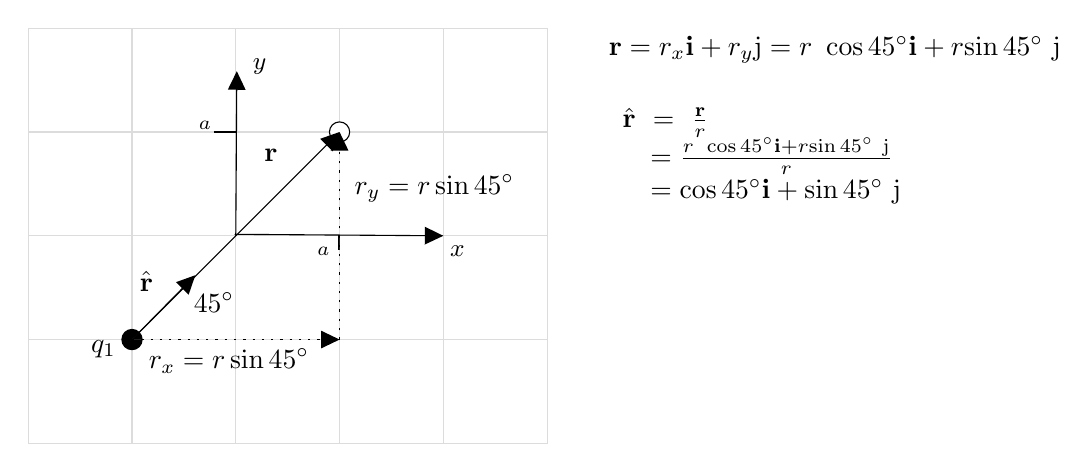
\begin{tikzpicture}[x=0.75pt,y=0.75pt,yscale=-1,xscale=1]
%uncomment if require: \path (0,227); %set diagram left start at 0, and has height of 227

%Shape: Grid [id:dp529276453314883] 
\draw  [draw opacity=0] (22.5,12) -- (272.5,12) -- (272.5,212) -- (22.5,212) -- cycle ; \draw  [color={rgb, 255:red, 220; green, 220; blue, 220 }  ,draw opacity=1 ] (72.5,12) -- (72.5,212)(122.5,12) -- (122.5,212)(172.5,12) -- (172.5,212)(222.5,12) -- (222.5,212) ; \draw  [color={rgb, 255:red, 220; green, 220; blue, 220 }  ,draw opacity=1 ] (22.5,62) -- (272.5,62)(22.5,112) -- (272.5,112)(22.5,162) -- (272.5,162) ; \draw  [color={rgb, 255:red, 220; green, 220; blue, 220 }  ,draw opacity=1 ] (22.5,12) -- (272.5,12) -- (272.5,212) -- (22.5,212) -- cycle ;
%Straight Lines [id:da9891788651841897] 
\draw    (122.5,112) -- (122.98,35.71) ;
\draw [shift={(123,32.71)}, rotate = 90.36] [fill={rgb, 255:red, 0; green, 0; blue, 0 }  ][line width=0.08]  [draw opacity=0] (8.93,-4.29) -- (0,0) -- (8.93,4.29) -- cycle    ;
%Straight Lines [id:da2531333242243323] 
\draw    (122,111.29) -- (219.5,111.98) ;
\draw [shift={(222.5,112)}, rotate = 180.41] [fill={rgb, 255:red, 0; green, 0; blue, 0 }  ][line width=0.08]  [draw opacity=0] (8.93,-4.29) -- (0,0) -- (8.93,4.29) -- cycle    ;
%Shape: Circle [id:dp928405560720714] 
\draw  [fill={rgb, 255:red, 0; green, 0; blue, 0 }  ,fill opacity=1 ] (67.63,162) .. controls (67.63,159.31) and (69.81,157.13) .. (72.5,157.13) .. controls (75.19,157.13) and (77.37,159.31) .. (77.37,162) .. controls (77.37,164.69) and (75.19,166.87) .. (72.5,166.87) .. controls (69.81,166.87) and (67.63,164.69) .. (67.63,162) -- cycle ;
%Shape: Circle [id:dp5390897406789283] 
\draw  [fill={rgb, 255:red, 255; green, 255; blue, 255 }  ,fill opacity=1 ] (167.63,62) .. controls (167.63,59.31) and (169.81,57.13) .. (172.5,57.13) .. controls (175.19,57.13) and (177.37,59.31) .. (177.37,62) .. controls (177.37,64.69) and (175.19,66.87) .. (172.5,66.87) .. controls (169.81,66.87) and (167.63,64.69) .. (167.63,62) -- cycle ;
%Straight Lines [id:da7315731890311423] 
\draw    (172.25,118.64) -- (172.25,111.64) ;
%Straight Lines [id:da41456511159458476] 
\draw    (112,62) -- (122.5,62) ;
%Straight Lines [id:da2368656312096422] 
\draw [fill={rgb, 255:red, 255; green, 255; blue, 255 }  ,fill opacity=1 ]   (72.5,162) -- (170.38,64.12) ;
\draw [shift={(172.5,62)}, rotate = 135] [fill={rgb, 255:red, 0; green, 0; blue, 0 }  ][line width=0.08]  [draw opacity=0] (8.93,-4.29) -- (0,0) -- (8.93,4.29) -- cycle    ;
%Straight Lines [id:da7182242007176092] 
\draw [fill={rgb, 255:red, 255; green, 255; blue, 255 }  ,fill opacity=1 ]   (72.5,162) -- (100.9,133.14) ;
\draw [shift={(103,131)}, rotate = 134.54] [fill={rgb, 255:red, 0; green, 0; blue, 0 }  ][line width=0.08]  [draw opacity=0] (8.93,-4.29) -- (0,0) -- (8.93,4.29) -- cycle    ;
%Straight Lines [id:da30412883702424365] 
\draw [fill={rgb, 255:red, 255; green, 255; blue, 255 }  ,fill opacity=1 ] [dash pattern={on 0.84pt off 2.51pt}]  (72.5,162) -- (169.5,162) ;
\draw [shift={(172.5,162)}, rotate = 180] [fill={rgb, 255:red, 0; green, 0; blue, 0 }  ][line width=0.08]  [draw opacity=0] (8.93,-4.29) -- (0,0) -- (8.93,4.29) -- cycle    ;
%Straight Lines [id:da8752471532648969] 
\draw [fill={rgb, 255:red, 255; green, 255; blue, 255 }  ,fill opacity=1 ] [dash pattern={on 0.84pt off 2.51pt}]  (172.5,162) -- (172.5,65) ;
\draw [shift={(172.5,62)}, rotate = 90] [fill={rgb, 255:red, 0; green, 0; blue, 0 }  ][line width=0.08]  [draw opacity=0] (8.93,-4.29) -- (0,0) -- (8.93,4.29) -- cycle    ;

% Text Node
\draw (129.5,25.4) node [anchor=north west][inner sep=0.75pt]  [font=\small]  {$y$};
% Text Node
\draw (224.5,115.4) node [anchor=north west][inner sep=0.75pt]  [font=\small]  {$x$};
% Text Node
\draw (160.5,116.4) node [anchor=north west][inner sep=0.75pt]  [font=\scriptsize]  {$a$};
% Text Node
\draw (103.5,55.4) node [anchor=north west][inner sep=0.75pt]  [font=\scriptsize]  {$a$};
% Text Node
\draw (135,69) node [anchor=north west][inner sep=0.75pt]   [align=left] {$\displaystyle \mathbf{r}$};
% Text Node
\draw (51.5,161) node [anchor=north west][inner sep=0.75pt]   [align=left] {$\displaystyle q_{1}$};
% Text Node
\draw (75,128) node [anchor=north west][inner sep=0.75pt]   [align=left] {$\displaystyle \hat{\mathbf{r}}$};
% Text Node
\draw (178.5,81) node [anchor=north west][inner sep=0.75pt]   [align=left] {$\displaystyle r_{y} =r\sin 45^{\circ }$};
% Text Node
\draw (79.37,165) node [anchor=north west][inner sep=0.75pt]   [align=left] {$\displaystyle r_{x} =r\sin 45^{\circ }$};
% Text Node
\draw (101,138) node [anchor=north west][inner sep=0.75pt]   [align=left] {$\displaystyle 45^{\circ }$};
% Text Node
\draw (301,47.4) node [anchor=north west][inner sep=0.75pt]    {$ \begin{array}{l}
\hat{\mathbf{r}} \ =\ \frac{\mathbf{r}}{r}\\
\ \ \ =\frac{r\ \cos 45\mathbf{^{\circ } i} +r\mathrm{\sin 45^{\circ } \ j}}{r}\\
\ \ \ =\cos 45\mathbf{^{\circ } i} +\mathrm{\sin 45^{\circ } \ j}
\end{array}$};
% Text Node
\draw (301,14.4) node [anchor=north west][inner sep=0.75pt]    {$\mathbf{r} =r_{x}\mathbf{i} +r_{y}\mathrm{j} =r\ \cos 45\mathbf{^{\circ } i} +r\mathrm{\sin 45^{\circ } \ j}$};


\end{tikzpicture}


Substitution gives

\begin{equation}
\bfvec{E}_{\text{at }(a,a)\text{ due to }q_1}=kq_1\frac{1}{r^2}\rhat = kq_1\frac{1}{8a^2}(\cos 45^\circ \ihat + \sin 45^\circ \jhat) =\frac{kq_1}{8a^2}\left[\frac{1}{\sqrt{2}}\ihat + \frac{1}{\sqrt{2}}\jhat\right]\thinspace,
\end{equation}

which is the same result obtained in the previous example, as expected.

To calculate $\bfvec{E}$, we can use

\begin{equation}
|\bfvec{E}|=E=\sqrt{E_x^2+E_y^2}
\end{equation}

and plug in $E_x=k\frac{q_1}{8a^2}\frac{1}{\sqrt{2}}$ and $E_y=k\frac{q_1}{8a^2}\frac{1}{\sqrt{2}}$ and use $\sqrt{c^2}=|c|$ (where $c$ is a real number) to show that $E=k|q_1|/{8a^2}$. There is an easier way. Taking the magnitude of both sides of

$\ds\bfvec{E}=kq_1\frac{\rhat}{r^2}\quad$
gives
$\quad\ds|\bfvec{E}|=k|q_1|\frac{|\rhat|}{r^2}$.

The magnitude of a unit vector is $1$, so

$\ds|\bfvec{E}|=k|q_1|\frac{1}{r^2}=\frac{k|q_1|}{8a^2},\thickspace$ as before.

\section{Problem II}

Charge $q_1$ is at $(x,y)=(-a,a)$. Find the electric field at $(x,y)=(a, 0)$ using $\bfvec{E}_{\text{at }(a,0)\text{ due to }q_1}=kq_1{\rhat}/{r^2}$. Check signs of the components of $\bfvec{E}$ using the technique used in Example I. Also, find $E$.

\input{../Electric_Force/figures/grid.tikz}

\ifsolutions
{\bf Answer}:

$\bfvec{r}=2a\ihat-a\jhat$,
$\quad$
$\ds\rhat=\frac{2}{\sqrt{5}}\ihat-\frac{1}{\sqrt{5}}\jhat$,
$\quad$ $r^2=5a^2$

$\ds\bfvec{E}_{\text{at }(a,0) \text{ due to }q_1}=\frac{kq_1}{5a^2}\left(\frac{2}{\sqrt{5}}\ihat -\frac{2}{\sqrt{5}}\jhat\right)$, which matches the solution to Problem I, as expected.
\fi

\newpage

\section{Problem III - Superposition}

In the previous examples, only one charge was responsible for creating the electric field $\bfvec{E}$. When there are more charges, superposition can be used to find the total electric field by summing $\bfvec{E}$ due to each charge.

Charge $q_1 = +q$ is at $(x, y) = (a, 0)$, charge $q_2 = +q$ is at $(x, y) = (-a, 0)$, and charge $q_3 = -q$ is at $(x, y) = (0, a)$. Assume that $q$ is a positive number.

\begin{enumerate}

  \item Draw this charge configuration below.

\end{enumerate}

\ifsolutions



\tikzset{every picture/.style={line width=0.75pt}} %set default line width to 0.75pt        

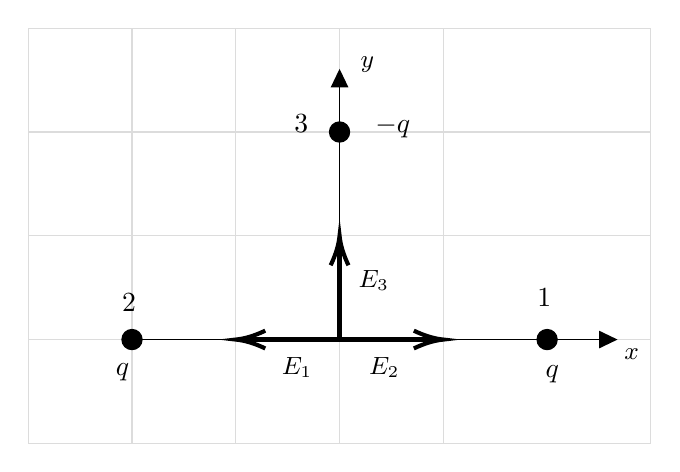
\begin{tikzpicture}[x=0.75pt,y=0.75pt,yscale=-1,xscale=1]
%uncomment if require: \path (0,200); %set diagram left start at 0, and has height of 200

%Shape: Grid [id:dp331631089200787] 
\draw  [draw opacity=0] (0,0) -- (300,0) -- (300,200) -- (0,200) -- cycle ; \draw  [color={rgb, 255:red, 220; green, 220; blue, 220 }  ,draw opacity=1 ] (50,0) -- (50,200)(100,0) -- (100,200)(150,0) -- (150,200)(200,0) -- (200,200) ; \draw  [color={rgb, 255:red, 220; green, 220; blue, 220 }  ,draw opacity=1 ] (0,50) -- (300,50)(0,100) -- (300,100)(0,150) -- (300,150) ; \draw  [color={rgb, 255:red, 220; green, 220; blue, 220 }  ,draw opacity=1 ] (0,0) -- (300,0) -- (300,200) -- (0,200) -- cycle ;
%Straight Lines [id:da14224998842180447] 
\draw    (50,150) -- (280.93,150) ;
\draw [shift={(283.93,150)}, rotate = 180] [fill={rgb, 255:red, 0; green, 0; blue, 0 }  ][line width=0.08]  [draw opacity=0] (8.93,-4.29) -- (0,0) -- (8.93,4.29) -- cycle    ;
%Straight Lines [id:da6009743108133081] 
\draw    (150,150) -- (150,22.58) ;
\draw [shift={(150,19.58)}, rotate = 90] [fill={rgb, 255:red, 0; green, 0; blue, 0 }  ][line width=0.08]  [draw opacity=0] (8.93,-4.29) -- (0,0) -- (8.93,4.29) -- cycle    ;
%Shape: Circle [id:dp897042553915123] 
\draw  [fill={rgb, 255:red, 0; green, 0; blue, 0 }  ,fill opacity=1 ] (145.13,50) .. controls (145.13,47.31) and (147.31,45.13) .. (150,45.13) .. controls (152.69,45.13) and (154.87,47.31) .. (154.87,50) .. controls (154.87,52.69) and (152.69,54.87) .. (150,54.87) .. controls (147.31,54.87) and (145.13,52.69) .. (145.13,50) -- cycle ;
%Shape: Circle [id:dp06513064206546715] 
\draw  [fill={rgb, 255:red, 0; green, 0; blue, 0 }  ,fill opacity=1 ] (45.13,150) .. controls (45.13,147.31) and (47.31,145.13) .. (50,145.13) .. controls (52.69,145.13) and (54.87,147.31) .. (54.87,150) .. controls (54.87,152.69) and (52.69,154.87) .. (50,154.87) .. controls (47.31,154.87) and (45.13,152.69) .. (45.13,150) -- cycle ;
%Shape: Circle [id:dp6444706106350273] 
\draw  [fill={rgb, 255:red, 0; green, 0; blue, 0 }  ,fill opacity=1 ] (245.13,150) .. controls (245.13,147.31) and (247.31,145.13) .. (250,145.13) .. controls (252.69,145.13) and (254.87,147.31) .. (254.87,150) .. controls (254.87,152.69) and (252.69,154.87) .. (250,154.87) .. controls (247.31,154.87) and (245.13,152.69) .. (245.13,150) -- cycle ;
%Straight Lines [id:da4590810247872239] 
\draw [line width=1.5]    (150,150) -- (103,150) ;
\draw [shift={(100,150)}, rotate = 360] [color={rgb, 255:red, 0; green, 0; blue, 0 }  ][line width=1.5]    (14.21,-4.28) .. controls (9.04,-1.82) and (4.3,-0.39) .. (0,0) .. controls (4.3,0.39) and (9.04,1.82) .. (14.21,4.28)   ;
%Straight Lines [id:da5899954170232251] 
\draw [line width=1.5]    (150,150) -- (197,150) ;
\draw [shift={(200,150)}, rotate = 180] [color={rgb, 255:red, 0; green, 0; blue, 0 }  ][line width=1.5]    (14.21,-4.28) .. controls (9.04,-1.82) and (4.3,-0.39) .. (0,0) .. controls (4.3,0.39) and (9.04,1.82) .. (14.21,4.28)   ;
%Straight Lines [id:da04145943004324493] 
\draw [line width=1.5]    (150,150) -- (150,103) ;
\draw [shift={(150,100)}, rotate = 90] [color={rgb, 255:red, 0; green, 0; blue, 0 }  ][line width=1.5]    (14.21,-4.28) .. controls (9.04,-1.82) and (4.3,-0.39) .. (0,0) .. controls (4.3,0.39) and (9.04,1.82) .. (14.21,4.28)   ;

% Text Node
\draw (166,41.4) node [anchor=north west][inner sep=0.75pt]    {$-q$};
% Text Node
\draw (41,160.4) node [anchor=north west][inner sep=0.75pt]    {$q$};
% Text Node
\draw (248,161.4) node [anchor=north west][inner sep=0.75pt]    {$q$};
% Text Node
\draw (285.93,153.4) node [anchor=north west][inner sep=0.75pt]  [font=\small]  {$x$};
% Text Node
\draw (158.93,12.4) node [anchor=north west][inner sep=0.75pt]  [font=\small]  {$y$};
% Text Node
\draw (244,124.4) node [anchor=north west][inner sep=0.75pt]    {$1$};
% Text Node
\draw (44,126.4) node [anchor=north west][inner sep=0.75pt]    {$2$};
% Text Node
\draw (127,40.4) node [anchor=north west][inner sep=0.75pt]    {$3$};
% Text Node
\draw (120.93,157.4) node [anchor=north west][inner sep=0.75pt]  [font=\small]  {$E_{1}$};
% Text Node
\draw (162.93,157.4) node [anchor=north west][inner sep=0.75pt]  [font=\small]  {$E_{2}$};
% Text Node
\draw (157.93,115.4) node [anchor=north west][inner sep=0.75pt]  [font=\small]  {$E_{3}$};


\end{tikzpicture}

\else

\input{../Electric_Force/figures/grid.tikz}
\fi
\ifsolutions\else
\input{../Electric_Force/figures/grid.tikz}
\fi

\begin{enumerate}

  \item[2.] Why does it not make sense to ask what the electric \emph{force} is at the origin?

\end{enumerate}

\ifsolutions
There is no charge at the origin. (The electric field can be used to find the force on a charge \emph{if} it was placed at the origin.)
\else

\vskip 24pt
\fi
\ifsolutions\else
\vskip 24pt
\fi

In the following, 

\begin{enumerate}

  \item[3.] Find the electric field at the origin due to $q_1$. Write your answer in the form $\bfvec{E}_1=E_{x1}\ihat + E_{y1}\jhat$.

            \ifsolutions
            {\bf Answer}: $\ds\bfvec{E}_1=-\frac{kq}{a^2}\ihat$
            \else

            \vskip 72pt
            \fi
            \ifsolutions\else
            \vskip 72pt
            \fi

  \item[4.] Find the electric field at the origin due to $q_2$. Write your answer in the form $\bfvec{E}_2=E_{x2}\ihat + E_{y2}\jhat$.

            \ifsolutions
            {\bf Answer}: $\ds\bfvec{E}_2=+\frac{kq}{a^2}\ihat$
            \else

            \vskip 72pt
            \fi
            \ifsolutions\else
            \vskip 72pt
            \fi

  \item[5.] Find the electric field at the origin due to $q_3$. Write your answer in the form $\bfvec{E}_3=E_{x3}\ihat + E_{y3}\jhat$.

            \ifsolutions
            {\bf Answer}: $\ds\bfvec{E}_3=+\frac{kq}{a^2}\jhat$
            \else

            \vskip 72pt
            \fi
            \ifsolutions\else
            \vskip 72pt
            \fi

  \item[6.] Find the total electric field at the origin by adding $\bfvec{E}_1$, $\bfvec{E}_2$, and $\bfvec{E}_3$. Write your answer in the form $\bfvec{E}=E_{x}\ihat + E_{y}\jhat$.

            \ifsolutions
            {\bf Answer}: $\ds\bfvec{E}=+\frac{kq}{a^2}\jhat$
            \else

            \vskip 72pt
            \fi
            \ifsolutions\else
            \vskip 72pt
            \fi

  \item[7.] Will your answers to 3.--6. change if the problem had asked for the electric field at a different position? If so, which answers?

            \ifsolutions
            Yes, all answers. The electric field at a given location due to each charge depends on the distance to the location. If the location changes, the distance changes.
            \else

            \vskip 72pt
            \fi
            \ifsolutions\else
            \vskip 72pt
            \fi

  \item[8.] Find the electric field at the origin if charge $q_1=2q$ (instead of $q$).

            \ifsolutions
            {\bf Answer}: $\ds\bfvec{E}=-\frac{kq}{a^2}\ihat+\frac{kq}{a^2}\jhat$
            \else

            \vskip 72pt
            \fi
            \ifsolutions\else
            \vskip 72pt
            \fi

  \item[9.] Find the electric field at the origin if charge $q_1=-2q$ (instead of $q$).

            \ifsolutions
            {\bf Answer}: $\ds\bfvec{E}=+\frac{3kq}{a^2}\ihat+\frac{kq}{a^2}\jhat$
            \else

            \vskip 72pt
            \fi
            \ifsolutions\else
            \vskip 72pt
            \fi

\end{enumerate}

\end{document}